\section{Training algorithm}\label{sec:supp_algorithm}
\begin{algorithm}
	\caption{ANT Optimisation}
	\label{alg:growth}
	\scriptsize
	\begin{algorithmic}
		%\Require Topology $\mathbb{T}$, parameters $\theta$
		\State Initialise topology $\mathbb{T}$ and parameters $\mathbb{O}$\Comment{$\mathbb{T}$ is set to a root node with one solver and one transformer}
		\State Optimise parameters in $\mathbb{O}$ via gradient descent on NLL \Comment{Learning root classifier}
		\State Set the root node ``suboptimal"
		
		\While{true} \Comment{Growth of $\mathbb{T}$ begins}
		\State Freeze all parameters $\mathbb{O}$
		\State Pick next ``suboptimal'' leaf node $l\in\mathcal{N}_{leaf}$ in the breadth-first order
		%\State Add (1) linear classifier to $leaf$ and train new parameters?
		\State Add (1) router to $l$ and train new parameters \Comment{Split data}
		\State Add (2) transformer to $l$ and train new parameters\Comment{Deepen transform}
		\State Add (1) or (2) to $\mathbb{T}$ if validation error decreases, otherwise set $l$ to ``optimal''
		\State Add any new modules to $\mathbb{O}$ 
		%\State $b\gets r$
		%\State $r\gets a\bmod b$
		\If{no ``suboptimal'' leaves remain}
		\State Break
		\EndIf
		\EndWhile
		\State Unfreeze and train all parameters in $\mathbb{O}$\Comment{Global refinement with fixed $\mathbb{T}$}
	\end{algorithmic}
\end{algorithm}


%\begin{algorithm}
%	\caption{ANT Optimisation}
%	\label{alg:growth}
%	\small
%	\begin{algorithmic}
%		%\Require Topology $\mathbb{T}$, parameters $\theta$
%		\State Initialise topology $\mathbb{T}$ and parameters $\mathbb{O}$\Comment{$\mathbb{T}$ is set to a single root node and an incoming edge with input.}
%		\State Freeze all parameters $\mathbb{O}$
%		\While{true}
%		\State Pick next ``suboptimal'' $leaf$ to grow via breadth-first search
%		%\State Add (1) linear classifier to $leaf$ and train new parameters?
%		\State Add (1) router to $leaf$ and train new parameters\Comment{Splitting the node}
%		\State Add (2) transformer to $leaf$ and train new parameters\Comment{Deepening the node}
%		\State Add (1) or (2) permanently to $\mathbb{T}$ based if validation error decreases, otherwise leaf is ``optimal''
%		\State Add any new parameters to $\mathbb{O}$ and freeze
%		%\State $b\gets r$
%		%\State $r\gets a\bmod b$
%		\If{no ``suboptimal'' leaves remain}
%		\State Break
%		\EndIf
%		\EndWhile
%		\State Unfreeze and train all parameters $\mathbb{O}$\Comment{$\mathbb{T}$ is fixed during refinement}
%	\end{algorithmic}
%\end{algorithm}
\vspace{-2mm}
\section{Additional related work}\label{sec:supp_related_work}
Here we provide an expanded review of related works, precluded from the main text due to space limit. The tree-structure of ANTs naturally performs conditional computation. We can also view the proposed tree-building algorithm as a form of neural architecture search. We provide surveys of these areas and their relations to ANTs.

\textbf{Conditional Computation:} in NNs, computation of each sample engages every parameter of the model. In contrast, DTs route each sample to a single path, only activating a small fraction of the model. \citet{bengio2013deep} advocated for this notion of conditional computation to be integrated into NNs, and this has become a topic of growing interest. Rationales for using conditional computation ranges from attaining better capacity-to-computation ratio \citep{bengio2013estimating,davis2013low,bengio2015conditional,Shazeer2017OutrageouslyLN} to adapting the required computation to the difficulty of the input and task \citep{bengio2015conditional,almahairi2016dynamic,Teerapittayanon2016BranchyNetFI,Graves2016AdaptiveCT,Figurnov2017SpatiallyAC,veit2017convolutional}. We view the growth procedure of ANTs as having a similar motivation with the latter---processing raw pixels is suboptimal for computer vision tasks, but we have no reason to believe that the hundreds of convolutional layers in current state-of-the-art architectures \citep{he2016deep,huang2017densely} are necessary either. Growing ANTs adapts the architecture complexity to the dataset as a whole, with routers determining the computation needed on a per-sample basis. 
% (Kai): Standard NNs can be thought of as computation graphs in which any data sample is passed through the same sequence of computations. In contrast, DTs do not modify the data, but instead route different samples down different paths, allowing each path to be lightweight. Bengio \citep{bengio2013deep} advocated for this property of conditional computation to be integrated into NNs, and this has become a topic of growing interest. There are many motivations for using conditional computation in NNs, from creating gated mixture-of-experts models \citep{bengio2013estimating,davis2013low,bengio2015conditional,Shazeer2017OutrageouslyLN} to minimising the amount of computation needed in a data-dependent fashion 
%\citep{bengio2015conditional,almahairi2016dynamic,Teerapittayanon2016BranchyNetFI,Graves2016AdaptiveCT,Figurnov2017SpatiallyAC,veit2017convolutional}.
%We share motivations with adaptive computation time, a form of conditional computation in which the amount of computation grows with the difficulty of the input data and task \citep{Graves2016AdaptiveCT}. We view the growth procedure of ANTs as having a similar motivation---processing raw pixels is suboptimal for computer vision tasks, but we have no reason to believe that the hundreds of convolutional layers in current state-of-the-art architectures \citep{he2016deep,huang2017densely} are necessary either. Growing ANTs adapts the complexity of the architecture to the dataset as a whole, with routers determining the amount of computation needed on a per-sample basis.

\textbf{Neural Architecture Search:} the ANT growing procedure is related to the progressive growing of NNs \citep{fahlman1990cascade,hinton2006fast,xiao2014errordriven,chen2016net2net,srivastava2015highway,lee2017lifelong,cai2018efficient,irsoy2018continuously}, or more broadly, the field of neural architecture search \citep{zoph2016neural,brock2017smash,cortes2017adanet}. This approach, mainly via greedy layerwise training, has historically been one solution to optimising NNs \citep{fahlman1990cascade,hinton2006fast}. However, nowadays it is possible to train NNs in an end-to-end fashion. One area which still uses progressive growing is lifelong learning, in which a model needs to adapt to new tasks while retaining performance on previous ones \citep{xiao2014errordriven,lee2017lifelong}. In particular, \citep{xiao2014errordriven} introduced a method that grows a tree-shaped network to accommodate new classes. However, their method never transforms the data before passing it to the children classifiers, and hence never benefit from the parent's representations. 

Whilst we learn the architecture of an ANT in a greedy, layerwise fashion, several other methods search globally. Based on a variety of techniques, including evolutionary algorithms \citep{stanley2002evolving,real2017large}, reinforcement learning \citep{zoph2016neural}, sequential optimisation \citep{liu2017progressive} and boosting \citep{cortes2017adanet}, these methods find extremely high-performance yet complex architectures. In our case, we constrain the search space to simple tree-structured NNs, retaining desirable properties of DTs such as data-dependent computation and interpretable structures, while keeping the space and time requirement of architecture search tractable thanks to the locality of our growth procedure.

\textbf{Cascaded trees and forests:} another noteworthy strand of work for feature learning with tree-structured models is cascaded forests---stacks of RFs where the outputs of intermediate models are fed into the subsequent ones \citep{montillo2011entangled,kontschieder2013geof,zhou2017deepft}. It has been shown how a cascade of DTs can be mapped to NNs with sparse connections \citep{sethi1990entropy}, and more recently \citet{richmond2015mapping} extended this argument to RFs. However, the features obtained in this approach are the intermediate outputs of respective component models, which are not optimised for the target task, and cannot be learned end-to-end, thus limiting its representational quality. Recently, \citet{feng2018multi} introduced a method to jointly train a cascade of gradient boosted trees (GBTs) to improve the limited representation learning ability of such previous work. A variant of target propagation \cite{lee2015difference} was designed to enable the end-to-end training of cascaded GBTs, each of which is non-differentiable and thus not amenable to back-propagation. 

%\citet{irsoy2018continuously} introduced (a) tunnel networks and (b) budding perceptrons. Tunnel networks add a highway connection \citep{srivastava2015highway} to internal nodes, allowing them to gate between pure residual \citep{he2016deep} and nonlinear operations. Budding perceptrons extend the bud node concept to potentially decompose internal nodes into their own trees, providing a way for the tree to grow on the inside. 


%\textbf{Alternative Computer Vision Architectures:} Although computer vision tasks are typically dominated by CNNs with fixed structures trained via backpropagation, some recent works have introduced alternatives that can be more robust, sample efficient, and effective at disentangling latent factors \citep{george2017generative,sabour2017dynamic,hinton2018matrix}. While ANTs are closer to traditional DT or mixture of experts models, dunno what I want to say...

\section{Set-up details}\label{sec:supp_train_details}
\vspace{-2mm}
\paragraph{Data:} we perform our experiments on the SARCOS robot inverse dynamics dataset\footnote{\url{http://www.gaussianprocess.org/gpml/data/}}, the MNIST digit classification task \citep{lecun1998gradient} and the CIFAR-10 object recognition task \citep{krizhevsky2009learning}. The SARCOS dataset consists of 44,484 training and 4,449 testing examples, where the goal is to map from the 21-dimensional input space (7 joint positions, 7 joint velocities and 7 joint accelerations) to the corresponding 7 joint torques \citep{vijayakumar2000locally}. No dataset preprocessing or augmentation is used. The MNIST dataset consists of $60,000$ training and $10,000$ testing examples, all of which are $28\times28$ grayscale images of digits from $0$ to $9$ ($10$ classes). The dataset is preprocessed by subtracting the mean, but no data augmentation is used. The CIFAR-10 dataset consists of $50,000$ training and $10,000$ testing examples, all of which are $32\times32$ coloured natural images drawn from $10$ classes. We adopt an augmentation scheme widely used in the literature \citep{goodfellow2013maxout,lin2013network,springenberg2014striving,he2016deep,huang2017densely} where images are zero-padded with 4 pixels on each side, randomly cropped and horizontally mirrored. For all three datasets, we hold out $10\%$ of training images as a validation set. The best model is selected based on the validation accuracy over the course of ANT training, spanning both the growth phase and the refinement phase, and its test accuracy is reported. 

\vspace{-5mm}
\paragraph{Training:} both the growth phase and the refinement phase of ANTs are performed on a single Titan X GPU on all three datasets. For all the experiments in this paper, we employ the following training protocol: (1) optimise parameters using Adam \citep{kingma2014adam} with initial learning rate of $10^{-3}$ and $\beta = [0.9, 0.999]$, with minibatches of size $512$; (2) during the growth phase, employ early stopping with a patience of $5$, that is, training is stopped after 5 epochs of no progress on the validation set; (3) during the refinement phase, train for $300$ epochs for SARCOS, $100$ epochs for MNIST and $200$ epochs for CIFAR-10, decreasing the learning rate by a factor of $10$ at every multiple of $50$. Training times are provided in Supp.~Sec.~\ref{sec:supp_traintime}.  

We observe that the patience level is an important hyperparameter which affects the quality of the growth phase; very low or high patience levels result in new modules underfitting or overfitting locally, thus preventing meaningful further growth and limiting the accuracy of the resultant models. We tuned this hyperparameter using the validation sets, and set the patience level to $5$, which produced consistently good performance on SARCOS, MNIST and CIFAR-10 datasets across different specifications of primitive modules. A quantitative evaluation on CIFAR-10 is given in Supp.~Sec.~\ref{sec:supp_effect_of_patience}.

In the SARCOS experiments, all the non-NN-based methods were trained using scikit-learn \citep{pedregosa2011scikit}. Hidden layers in the baseline MLPs are followed by tanh non-linearities and contain 256 units to be consistent with the complexity of transformer modules.

\vspace{-3mm}
\paragraph{Primitive modules:} we train ANTs with a range of primitive modules as shown in Tab.~2 in the main text. For simplicity, we define the modules based on three types of NN layers: convolutional, global-average-pooling (GAP) and fully-connected (FC). Solver modules are fixed as linear models e.g. linear classifier and linear regression. Router modules are binary classifiers with a sigmoid output. All convolutional and FC layer are followed by ReLU or tanh non-linearities, except in the last layers of solvers and routers. For image classification experiments, we also apply $2\times2$ max-pooling to feature maps after every $d$ transformer modules where $d$ is the downsample frequency. For the SARCOS regression experiment, hidden layers in the routers and transformers contain 256 units. We balance the number of parameters in the router and transformer modules to be of the same order of magnitude to avoid favouring either partitioning the data or learning more expressive features. 


% ------------------------ DO NOT DELETE --------------------------------
% %%% Table that shows the number of parameters for the ablation study %%%%%
% \section{Ablation study of different constituent modules}
% In this section, we investigate the roles of router and transformer modules on the performance of ANTs. 

% \begin{table}[h]
% 	\caption{Ablation study to compare the effects of different components of ANTs on the number of parameters\label{tab:ablationstudy_2}}
% 	\vspace{-2mm}
% 	\scriptsize
%     \center
% 	\begin{tabular}{|l|ccc|ccc|ccc|}
% 		\hline
% 		\multicolumn{1}{|c}{\textbf{Method}} &  \multicolumn{3}{|c|}{\textbf{Params. (Full)}} & \multicolumn{3}{|c|}{\textbf{Params. (Path)}} & \multicolumn{3}{c|}{\textbf{Params. (Path without routers)}}  \\
% 			& Default & No $\mathcal{R}$ & No $\mathcal{T}$ & Default & No $\mathcal{R}$ & No $\mathcal{T}$ & Default & No $\mathcal{R}$  & No $\mathcal{T}$ \\
% 		\hline
% 		ANT-MNIST-A & 101K & 82K & 74K & 85K & 82K & 22K & 49K & 82K & 8K\\
% 	    ANT-MNIST-B & 77K  & 54K & 57K & 51K & 54K & 15K & 44K & 54K & 8K\\
%         ANT-MNIST-C & 40K  & 3K  & 32K & 8K  &  3K &  9K & 6K  & 3K & 8K\\
% 		ANT-CIFAR10-A & 1.4M & 1.0M & 0.8M & 1.0M & 1.0M & 0.5M & 0.8M & 1.0M & 0.03M\\
%         ANT-CIFAR10-B & 0.9M & 0.6M & 0.4M & 0.6M & 0.6M & 0.2M & 0.4M & 0.6M & 0.03M\\
%         ANT-CIFAR10-C & 0.7M & 0.3M & 0.3M & 0.5M & 0.3M & 0.1M & 0.2M & 0.3M & $4\times 10^{-5}$M\\
% 		\hline
% % 		\hline
% % 		ANT-MNIST-A & 101K& 74K  & 82K  & 85K  &  22K    &  82K  & 49K  & 8K & 82K\\
% % 	    ANT-MNIST-B & 77K & 57K & 54K & 51K  & 15K &  54K   & 44K  & 8K & 54K\\
% %         ANT-MNIST-C & 40K & 32K &  3K& 8K   &  9K  &   3K  & 6K   & 8K & 3K\\
% % 		ANT-CIFAR10-A &1.4M & 0.8M   & 1.0M & 1.0M & 0.5M   & 1.0M & 0.8M & 0.03M &1.0M \\
% %         ANT-CIFAR10-B &0.9M & 0.4M  & 0.6M & 0.6M & 0.2M   & 0.6M & 0.4M  & 0.03M  & 0.6M\\
% %         ANT-CIFAR10-C &0.7M & 0.3M & 0.3M & 0.5M & 0.1M  & 0.3M & 0.2M  & $4\times 10^{-5}$M & 0.3M\\
% % 		\hline
% 	\end{tabular}
% 	\vspace{-2mm}
% \end{table}




% \begin{table}[h]
% 	\caption{Ablation study to compare the effects of different components of ANTs on the number of parameters\label{tab:ablationstudy_2}}
% 	\vspace{-2mm}
% 	\scriptsize
%     \center
% 	\begin{tabular}{|l|ccc|}
% 		\hline
% 		\multicolumn{1}{|c}{\textbf{Method}} &  \multicolumn{3}{|c|}{\textbf{Params. (Full)}} \\
% 			& Default & No $\mathcal{R}$ & No $\mathcal{T}$  \\
% 		\hline
% 		ANT-MNIST-A & 49K & 82K & 8K\\
% 	    ANT-MNIST-B & 44K & 54K & 8K\\
%         ANT-MNIST-C & 6K  & 3K & 8K\\
% 		ANT-CIFAR10-A & 0.8M & 1.0M & 0.03M\\
%         ANT-CIFAR10-B & 0.4M & 0.6M & 0.03M\\
%         ANT-CIFAR10-C & 0.2M & 0.3M & $4\times 10^{-5}$M\\
% 		\hline
% 	\end{tabular}
% 	\vspace{-2mm}
% \end{table}

\vspace{-2mm}
\section{Training times}\label{sec:supp_traintime}
\vspace{-2mm}
Tab. \ref{table:traintime} summarises the time taken on a single Titan X GPU for the growth phase and refinement phase of various ANTs, and compares against the training time of All-CNN \citep{springenberg2014striving}. Local optimisation during the growth phase means that the gradient computation is constrained to the newly added component of the graph, allowing us to grow a good candidate model under $3$ hours on one GPU. 
\begin{table}[ht]
	\vspace{-2mm}
	\footnotesize
	\caption{Training time comparison. Time and number of epochs taken for the growth and refinement phase are shown. along with the time required to train the baseline, All-CNN \citep{springenberg2014striving}.}
	\label{table:traintime}
	%\vskip 0.1in  % Was 0.15in
 	\vspace{-3mm}
	\begin{center}
		\begin{tabular}{l|c|c|c|c}
				\hline
				\multicolumn{1}{c}{} &  \multicolumn{2}{c}{\textbf{Growth}} & \multicolumn{2}{c}{\textbf{Fine-tune}}  \\
				\hline
				Model & Time & Epochs  & Time  & Epochs\\
				\hline
				%				\abovespace
				%				ANT-MNIST-1  &  &   &LC& 200 \\
				%				ANT-MNIST-2& &  & LC & 200\\
				%				ANT-MNIST-6 & &  &LC & 200 \\
				%				\hline
				%	\abovespace
				All-CNN (baseline)&--~~~ & --~~~ & 1.1 (hr) &200 \\
				ANT-CIFAR10-A&1.3 (hr) & 236  & 1.5 (hr) &200 \\
				ANT-CIFAR10-B & 0.8 (hr) & 313 & 0.9 (hr) & 200\\
				ANT-CIFAR10-C&  0.7 (hr) &  285& 0.8 (hr) & 200 \\
				\hline
		\end{tabular}
			%	\end{sc}

	\end{center}
 	\vspace{-7mm}
\end{table}


\begin{figure*}[ht]
    \vspace{-4mm}
	\center
	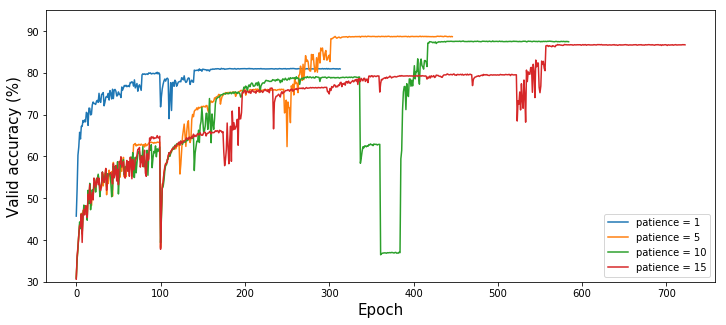
\includegraphics[width=0.7\linewidth]{figures/fig_patience.png}
    \vspace{-4mm}
	\caption{\small Effect of patience level on the validation accuracy trajectory during training. Each curve shows the validation accuracy on CIFAR-10 dataset.}
	\vspace{-4mm}
    \label{fig:patience}
\end{figure*}

\vspace{-2mm}
\section{Effect of training steps in the growth
\vspace{-2mm}
phase}\label{sec:supp_effect_of_patience}
Fig. \ref{fig:patience} compares the validation accuracies of the same ANT-CIFAR-C model trained on the CIFAR-10 dataset with varying levels of patience during early stopping in the growth phase. A higher patience level corresponds to more training epochs for optimising new modules in the growth phase. When the patience level is 1, the architecture growth terminates prematurely and plateaus at low accuracy at $80\%$. On the other hand, a patience level of 15 causes the model to overfit locally with  $87\%$. The patience level of 5 gives the best results with $91\%$ validation accuracy.

%A patience level of 1 leads the model to underfit with $80\%$ accuracy, while a patience level of 15 causes the model to overfit locally with  $87\%$ accuracy; in between these, the patience level of 5 gives the best results with a validation accuracy of $91\%$.}
%Figure. 1 shows that when too few steps of optimisation are performed e.g. patience level is 1, the architecture growth terminates prematurely and plateaus at low validation accuracy at 80\%, which is roughly 10\% lower than the best case with patience level of 5. On the other hand, if too many optimisation steps are taken e.g patience level 15, this causes the added component to overfit locally, and leads to nearly 4\% drop in accuracy. Tuning this hyperparameter of patience level is therefore integral to successful optimisations of ANTs.



\section{Expert specialisation}\label{sec:supp_expert_specialisation}
\vspace{-2mm}
We investigate if the learned routing strategy is meaningful by comparing the classification accuracy of our default path-wise inference against that of the predictions from the leaf node with the smallest reaching probability. Tab. \ref{tab:test_routers} shows that using the least likely ``expert" leads to a substantial drop in classification accuracy, down to close to that of random guess or even worse for large trees (ANT-MNIST-C and ANT-CIFAR10-C). This demonstrates that features in ANTs become specialised to the subsets of the partitioned input space at lower levels in the tree hierarchy. 

\begin{table}[h]
	\caption {Comparison of classification performance between the default single-path inference scheme and the prediction based on the least likely expert. \label{tab:test_routers} between the }
 	\vspace{-4mm}
    \footnotesize
    \center
	\begin{tabular}{|l|c|c|}
		\hline
		\multicolumn{1}{|c}{\textbf{Module Spec.}} &  \multicolumn{1}{|c|}{\textbf{Error \%}} & \multicolumn{1}{c|}{\textbf{Error \%}}  \\
		&(Selected path) & (Least likely path)  \\
		\hline
		ANT-MNIST-A &0.69 & 86.18  \\
	    ANT-MNIST-B &0.73 & 81.98  \\
        ANT-MNIST-C &1.68 & 98.84  \\
		ANT-CIFAR10-A & 8.32 & 74.28  \\
        ANT-CIFAR10-B & 9.18 & 89.74  \\
        ANT-CIFAR10-C & 9.34 & 97.52  \\
		\hline
	\end{tabular}
\end{table}
\vspace{-4mm}
\section{Visualisation of discovered architectures}\label{sec:supp_architectures}
\vspace{-2mm}
Fig. \ref{fig:architectures} shows ANT architectures discovered on the MNIST (i-iii) and CIFAR-10 (iv-vi) datasets. We observe three notable trends. Firstly, a large proportion of the learned routers separate examples based on their classes (red histograms) with very high confidence (blue histograms). The ablation study in Sec.~5.~1 (Tab.~4 in the main text) shows that such hierarchical clustering benefits predictive performance, while the conditional computation enables more lightweight inference (Tab.~3 in the main text). Secondly, most architectures learn a few levels of features before resorting to primarily splits. However, over half of the architectures (ii-v) still learn further representations beyond the first split. Secondly, all architectures are unbalanced. This reflects the fact that some groups of samples may be easier to classify than others. This property is reflected by traditional DT algorithms, but not ``neural'' tree-structured models with pre-specified architectures \citep{laptev2014convolutional,frosst2017distilling,kontschieder2015deep,ioannou2016decision}. 
\begin{figure*}[ht]
	\center
	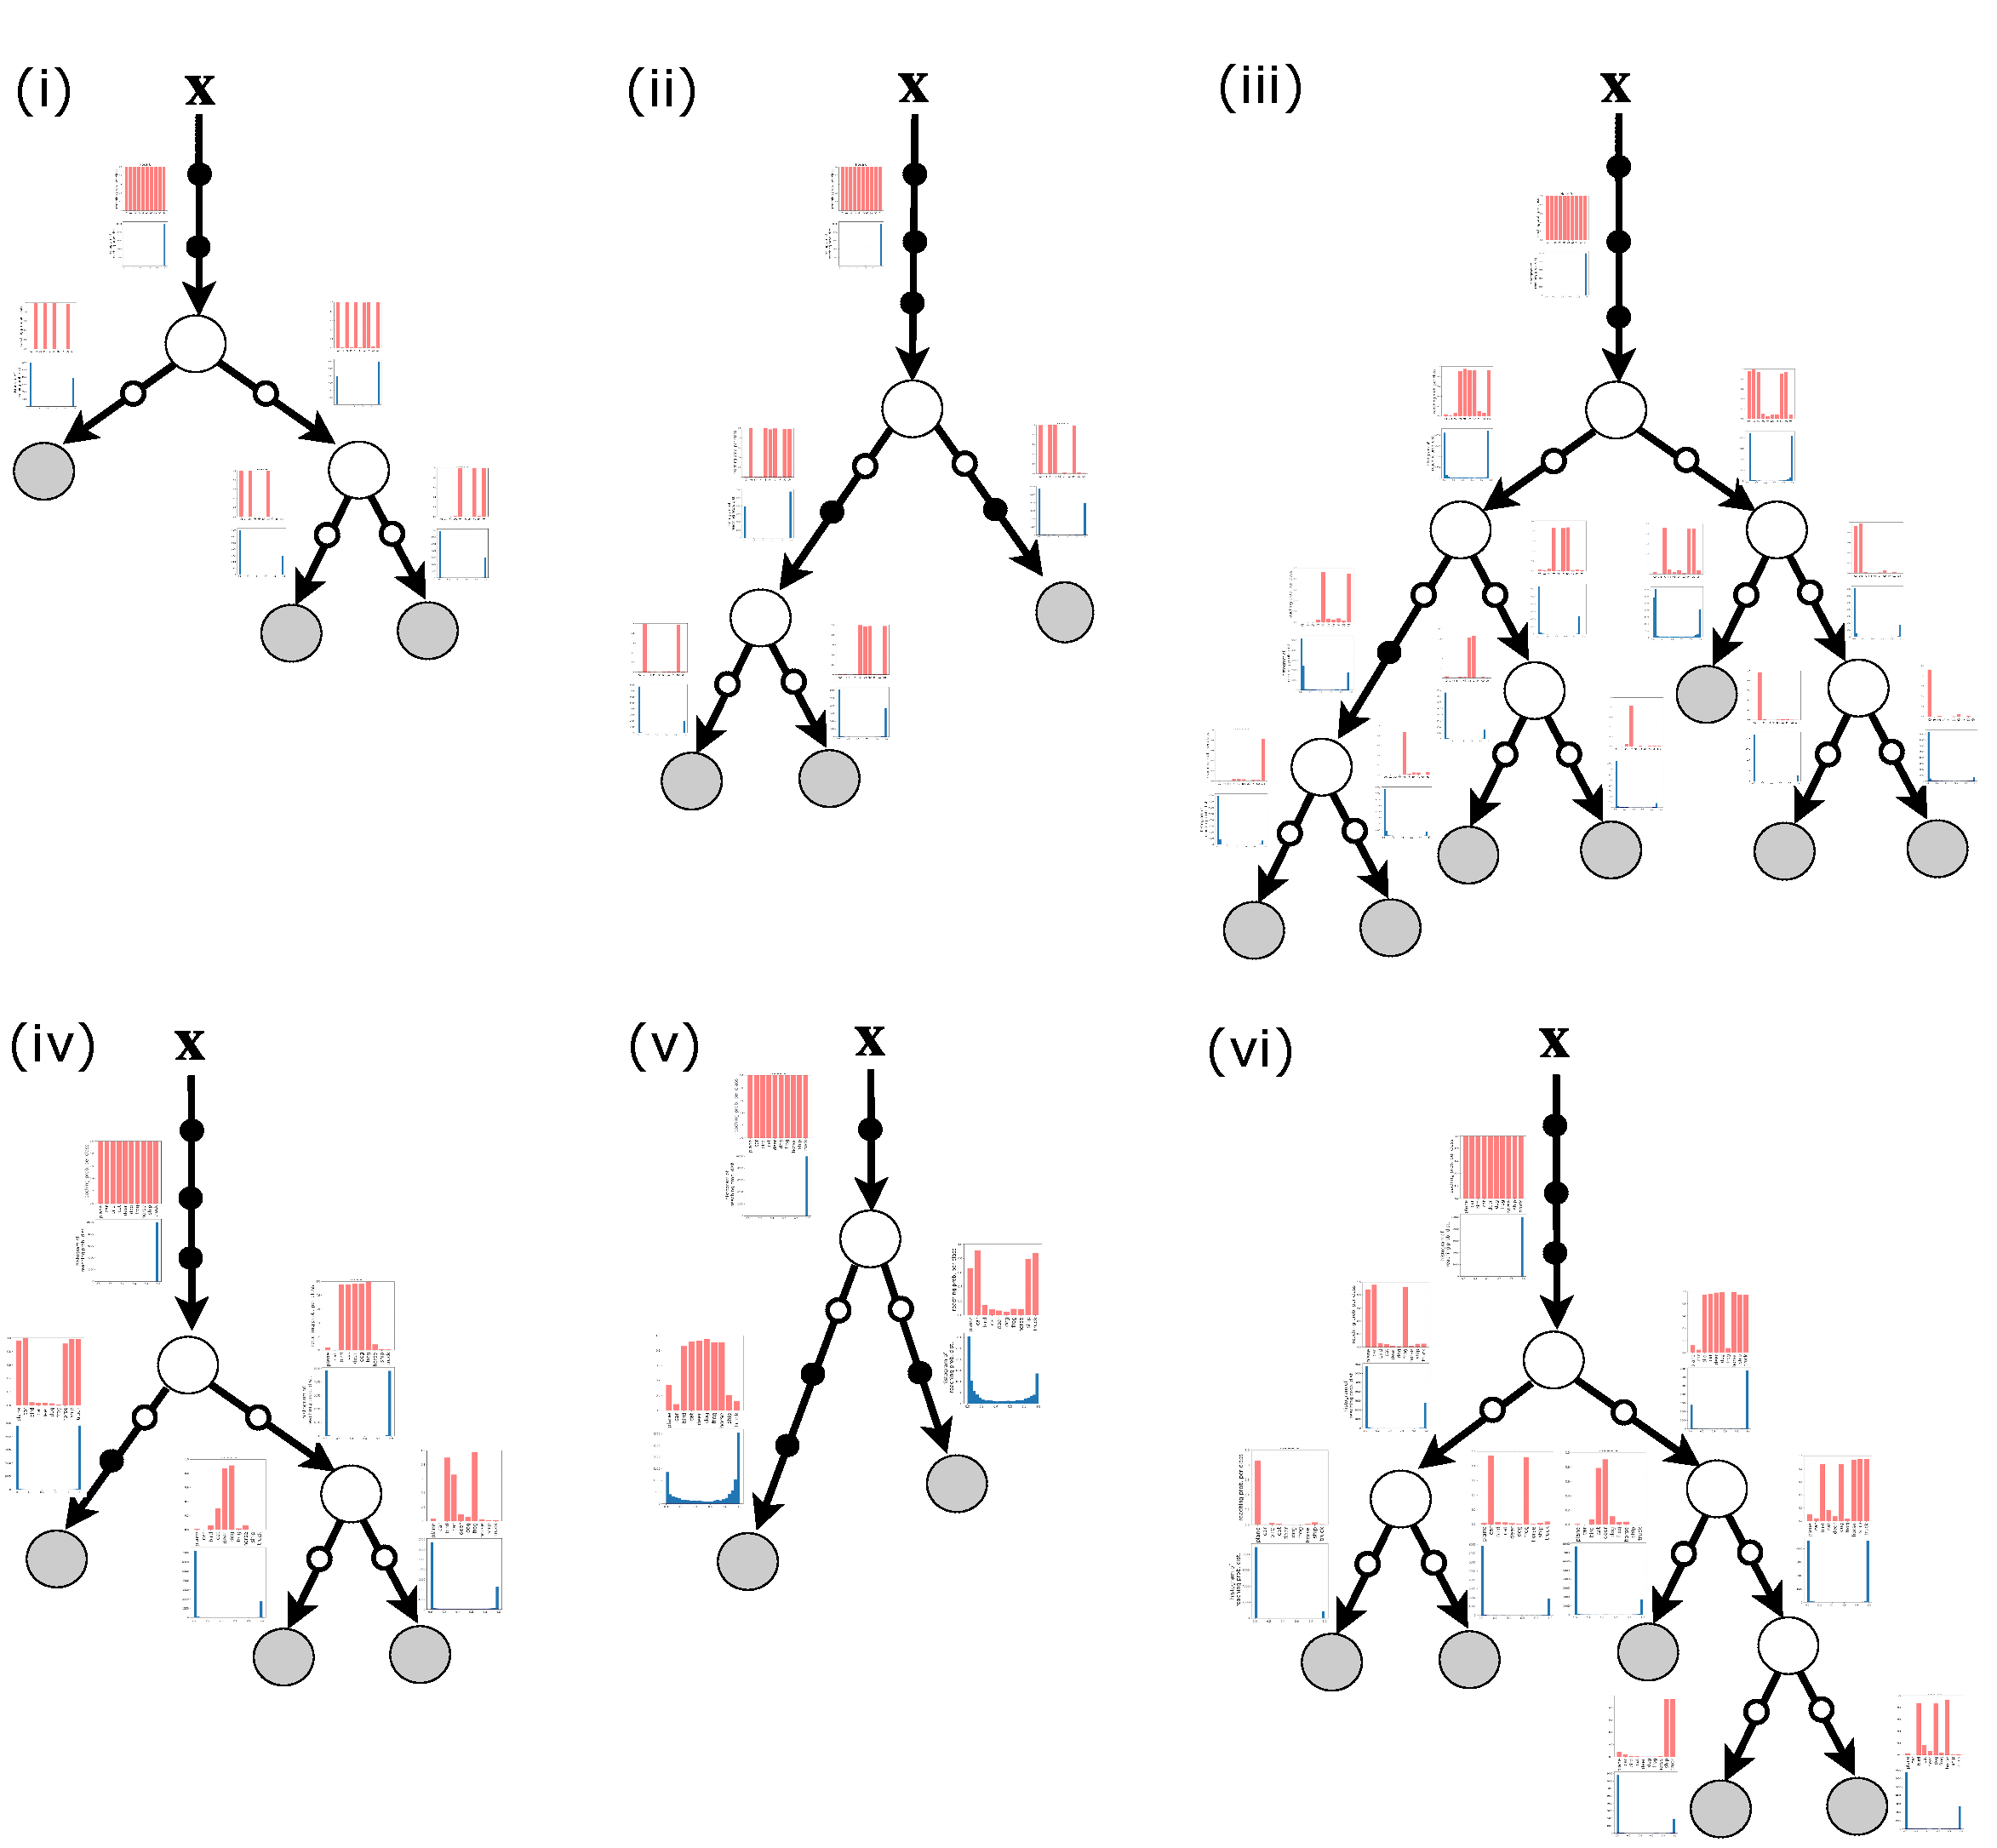
\includegraphics[width=0.8\linewidth]{figures/trees_all.pdf}
	\caption{\small Illustration of discovered ANT architectures. (i) ANT-MNIST-A, (ii) ANT-MNIST-B, (iii) ANT-MNIST-C, (iv) ANT-CIFAR10-A, (v) ANT-CIFAR10-B, (vi) ANT-CIFAR10-C. Histograms in red and blue show the class distributions and path probabilities at respective nodes. Small black circles on the edges represent transformers, circles in white at the internal nodes represent routers, and circles in gray are solvers. The small white circles on the edges denote specific cases where transformers are identity functions.}
	\label{fig:architectures}
\end{figure*}


% \section{Multivariate Regression}\label{sec:supp_regression}
% \vspace{-3mm}
% To demonstrate this, we also grow ANTs to perform (multivariate) regression on the SARCOS robot inverse dynamics dataset\footnote{\url{http://www.gaussianprocess.org/gpml/data/}}, which consists of 44,484 training and 4,449 testing examples, where the goal is to map from the 21-dimensional input space (7 joint positions, 7 joint velocities and 7 joint accelerations) to the corresponding 7 joint torques \citep{vijayakumar2000locally}. No dataset preprocessing or augmentation is used. We hold out 10\% of the training examples as a validation set. Baseline MLPs, routers and transformers are composed of single fully connected layers with 256 units with tanh nonlinearities, and the solver is a linear regressor. Other training details are the same as for classification (see Supp. Sec. \ref{sec:supp_train_details}). All non-NN-based methods were trained using scikit-learn \citep{pedregosa2011scikit}; only single-output GBT models were available so 7 separate GBTs were trained.

% The results are shown in Tab.~\ref{table:sarcos_results}. ANT-SARCOS outperforms all other methods in mean squared error with the full set of parameters, with GBTs performing slightly better using single-path inference. In comparison with results on MNIST and CIFAR-10, we note that the top 3 performing methods are all tree-based, with the third best method being an SDT (with MLP routers). This highlights the power of splitting the input space and conditional computation, both of which standard NNs are not capable of. Meanwhile, we still reap the benefits of representation learning, as shown by both ANT-SARCOS and the SDT (which is a specific form of ANT) requiring fewer parameters than the best-performing GBT configuration. Finally, we note that deeper NNs (5 vs. 3 hidden layers) can overfit on this small dataset, which makes the adaptive growth procedure of tree-based methods ideal for finding a model that exhibits good generalisation.

% \begin{table*}[ht]
% 	\caption{Comparison of performance of different models on SARCOS. The columns ``Error (Full)'' and ``Error (Path)'' indicate the mean squared error of predictions based on the full distribution and the single-path inference. The columns ``Params. (Full)'' and ``Params. (Path)'' respectively show the total number of parameters in the model and the average number of parameters utilised during single-path inference. ``Ensemble Size'' indicates the size of ensemble used to attain the reported accuracy. Results from \citet{zhao2017efficient} are included as a reference value from prior work, but are not directly comparable as they hold out 30\% of the training examples as a validation set.}
% 	\vspace{-3mm}
% 	\label{table:sarcos_results}
%     \center
%     \scriptsize
% 	\begin{tabular}{|c|l|cc|cc|c|}
% 		\hline
% 		& \multicolumn{1}{c|}{Method}
% 		& \multicolumn{1}{c}{\thead{\scriptsize Error \\ \scriptsize (Full)}}
% 		& \multicolumn{1}{c}{\thead{\scriptsize Error \\ \scriptsize (Path)}}
% 		& \multicolumn{1}{c}{\thead{\scriptsize Params. \\ \scriptsize (Full)}}
% 		& \multicolumn{1}{c|}{\thead{\scriptsize Params. \\ \scriptsize (Path)}}
% 		& \multicolumn{1}{c|}{\thead{\scriptsize Ensemble \\ \scriptsize Size}} \\	
% 		\hline
% 		\parbox[t]{2mm}{\multirow{11}{*}{\rotatebox[origin=c]{90}{SARCOS}}}
%         & Linear regression & 10.693 & N/A &\textbf{154}& N/A & 1 \\
%         & MLP with 2 hidden layers \citep{zhao2017efficient} & 5.111 & N/A & 31,804 & N/A & 1 \\
% 		& Decision tree & 3.708 & 3.708 & 319,591 & \textbf{25} & 1 \\
% 		& MLP with 1 hidden layer & 2.835 & N/A & 7,431 & N/A & 1 \\
%         & Gradient boosted trees & 2.661 & 2.661 & 391,324 & 2,083 & 7 $\times$ 30 \\
% 		& MLP with 5 hidden layers & 2.657 & N/A & 270,599 & N/A & 1 \\
% 		& Random forest & 2.426 & 2.426 & 40,436,840 & 4,791 & 200 \\
% 		& Random forest & 2.394 & 2.394 & 141,540,436 & 16,771 & 700 \\
% 		& MLP with 3 hidden layers & 2.129 & N/A & 139,015 & N/A & 1 \\
% 		&\cellcolor{gray!10}SDT (with MLP routers) &\cellcolor{gray!10} 2.118 &\cellcolor{gray!10} 2.246 &\cellcolor{gray!10} 28,045  &\cellcolor{gray!10} 10,167 &\cellcolor{gray!10} 1\\
% 		 & Gradient boosted trees & 1.444 & \textbf{1.444 }& 988,256 & 6,808 & 7 $\times$ 100 \\
% 		&\cellcolor{gray!10}ANT-SARCOS &\cellcolor{gray!10} \textbf{1.384} &\cellcolor{gray!10}  1.542 &\cellcolor{gray!10} 103,823  
% 		&\cellcolor{gray!10} 61,640 &\cellcolor{gray!10} 1\\
%       	\hline
% 	\end{tabular}
% \end{table*}

% \textbf{Ablation study:} we compare the regression error of our ANT in cases where the options for adding transformer or router modules are disabled (see Tab. \ref{tab:reg_ablationstudy}). In this experiment, patience levels are tuned separately for respective models. In the first case, the resulting models are equivalent to SDTs \citep{suarez1999globally} or HMEs \citep{jordan1994hierarchical} with locally grown architectures, while the second case is equivalent to standard NNs, grown adaptively layer by layer. We observe that either ablation consistently leads to higher regression errors across different module configurations. 
% \vspace{-3mm}
% \begin{table}[H]
% 	\caption{Ablation study to compare the effects of different components of ANTs on regression performance. ``NN'' refers to the case where the ANT is grown without routers while ``SDT/HME'' refers to the case where transformer modules on the edges are disabled. \label{tab:reg_ablationstudy}}
% 	\scriptsize
%     \center
% 	\begin{tabular}{|l|ccc|ccc|}
% 		\hline
% 		\multicolumn{1}{|c}{\textbf{Module Spec.}} &  \multicolumn{3}{|c|}{\textbf{Error (Full)}} & \multicolumn{3}{c|}{\textbf{ Error (Path)}} \\
% 			& ANT & NN & SDT/HME & ANT & NN & SDT/HME \\
% 			& (default) & (no routers) & (no transformers) & (default) & (no routers) & (no transformers) \\
% 		\hline
% 		ANT-SARCOS &1.384 & 2.511 & 2.118 &1.542 & 2.511 & 2.246 \\
% 		\hline
% 	\end{tabular}
% \end{table}
\vspace{-3mm}
\section{FLOPS}\label{sec:flops}
\vspace{-2mm}
Tab.\ref{tab:flops} reports the floating point operations per second (FLOPS) of ANT models for two inference schemes. The results for ResNet110 and DenseNet were retrieved from \cite{guan2017energy} and \cite{huang2018condensenet}, respectively. The FLOPs of all other models were computed using TorchStat toolbox available at \url{https://github.com/Swall0w/torchstat}. Using the single-inference reduces FLOPS in all ANT models to varying degrees.

\begin{table}[h]
% 	\caption {Comparison of classification performance between the default single-path inference scheme and the prediction based on the least likely expert. \label{tab:test_routers} between the }
    \caption{Comparison of FLOPs. \label{tab:flops}}
    \vspace{-5mm}
    \footnotesize
    \center
	\begin{tabular}{|c|l|c|c|}
		\hline
		&\multicolumn{1}{|c}{\textbf{Model}} &  \multicolumn{1}{|c|}{\textbf{FLOPS}} & \multicolumn{1}{c|}{\textbf{FLOPS}}  \\
		& &(multi-path) & (single-path)  \\
		\hline
		\parbox[t]{2mm}{\multirow{5}{*}{\rotatebox[origin=c]{90}{MNIST}}}
		&Linear Classifier & 8K & -   \\
		&LeNet-5 & 231 K & -  \\
		&ANT-MNIST-C & 99K & 83K  \\
	    &ANT-MNIST-B & 346K & 331K \\
        &ANT-MNIST-A & 382K & 380K  \\
        \hline
        
        \parbox[t]{2mm}{\multirow{7}{*}{\rotatebox[origin=c]{90}{CIFAR-10}}}&Net-in-Net & 222M &- \\
        &All-CNN & 245M & -\\
        &ResNet-110 & 256M&- \\
        &DenseNet-BC (k=24)& 9388M &- \\
		&ANT-CIFAR10-C & 66M & 61M  \\
        &ANT-CIFAR10-B & 163M & 149M  \\
        &ANT-CIFAR10-A & 254M & 243M  \\
		\hline
	\end{tabular}
\end{table}

\vspace{-5mm}
\section{Ensembling}\label{sec:supp_ensembling}
\vspace{-2mm}
As with traditional DTs \citep{breiman2001random} and NNs \citep{hansen1990neural}, ANTs can be ensembled to gain improved performance. In Tab.~\ref{tab:ensembling} we show the results of ensembling 8 ANTs (using the ``-A'' configurations for classification), each of which is trained with a randomly chosen split between training and validation sets. We compare against the single tree models, trained with the default split. In all cases both the multi-path and single-path inference performance is noticeably improved, and in MNIST we reach close to state-of-the-art performance (0.29\% versus 0.25\% \citep{sabour2017dynamic}) with significantly fewer parameters (851k versus 8.2M).
\vspace{-4mm}
\begin{table*}[ht]
	\caption{\small Comparison of prediction errors of a single ANT versus an ensemble of 8. \label{tab:ensembling}}
	\footnotesize
    \center
	\begin{tabular}{|l|cc|cc|cc|}
		\hline
		\multicolumn{1}{|c}{} &  \multicolumn{2}{|c|}{\textbf{MNIST} (Class Error \%)} &  \multicolumn{2}{|c|}{\textbf{CIFAR-10} (Class Error \%)} & \multicolumn{2}{c|}{\textbf{SARCOS} (MSE)}  \\
			& Multi-path & Single-path  & Multi-path & Single-path & Multi-path & Single-path   \\
		\hline
	    Single model & 0.64 & 0.69 & 8.31  & 8.32 & 1.384  & 1.542 \\	
        Ensemble & 0.29 & 0.30 & 7.76 & 7.79 & 1.226 & 1.372  \\
		\hline
	\end{tabular}
	\vspace{-4mm}
\end{table*}

\begin{table*}[ht]
	\caption{\small Parameter counts for a single ANT versus an ensemble of 8. \label{tab:ensembling_params}}
	\center
    \vspace{-1mm}
    \footnotesize
    \begin{tabular}{|l|cc|cc|cc|}
		\hline
		\multicolumn{1}{|c}{} &  \multicolumn{2}{|c|}{\textbf{MNIST} (No. Params.)} &  \multicolumn{2}{|c|}{\textbf{CIFAR-10} (No. Params.)} & \multicolumn{2}{c|}{\textbf{SARCOS}  (No. Params.)}  \\
			& Multi-path & Single-path  & Multi-path & Single-path & Multi-path & Single-path   \\
		\hline
	    Single model & 100,596 & 84,935 & 1.4M & 1.0M & 103,823 & 61,640 \\	
        Ensemble & 850,775 & 655,449 & 8.7M & 7.4M & 598,280 & 360,766  \\
		\hline
	\end{tabular}
	
	\vspace{-5mm}
\end{table*}

